\documentclass[a3paper,12pt]{article}
\title{\heiti ROMS公式笔记}
\author{\small 2017级海洋科学专业 崔英哲 \\ \small \url{https://github.com/Cuiyingzhe/OUC-Physical-Oceanography-Notes}}
\date{\small 2020.09.21}
\usepackage[UTF8]{ctex}
\usepackage{indentfirst}
\usepackage{geometry}
\usepackage{amsmath}
\usepackage{booktabs}
\usepackage{tabu}
\usepackage{caption}
%\usepackage{gensymb}
\usepackage{cite}
\usepackage{graphicx}
\usepackage{float}
\usepackage{hyperref}
\usepackage{cases}
\usepackage{esint}
\usepackage{fancyhdr}
\usepackage{CJK}
\usepackage{titlesec}
\usepackage{titletoc}
\usepackage{mathrsfs}
\usepackage{harpoon}
\usepackage{amssymb}
\usepackage{color}
\usepackage{bm}
\usepackage{framed}
\usepackage{setspace}
\usepackage{textcomp}
\usepackage{gensymb}    
\usepackage{tikz}
\usepackage{cancel}
\usepackage{multicol}
\newcommand*{\circled}[1]{\lower.7ex\hbox{\tikz\draw (0pt, 0pt)%
    circle (.5em) node {\makebox[1em][c]{\small #1}};}}
\newcommand*{\p}[2]{\frac{\partial #1}{\partial #2}}
%\usepackage[T1]{fontenc}
%\usepackage{mathptmx}
\hypersetup{
	colorlinks=true,
	linkcolor=black,
	citecolor=blue
}
\captionsetup[table]{labelsep=space,font={small}}
\captionsetup[figure]{labelsep=space,font={small}}
\geometry{a3paper,left=4cm,right=4cm,top=4cm,bottom=4cm}
\graphicspath{{D:/OUC/SRDP/notes/ROMS-Notes/figures/}}
\begin{document}
    \maketitle
    \renewcommand*\contentsname{}
    \tableofcontents
    \newpage
    \section{Ocean Model Formulation}
    \subsection{Equations of Motion}
    ROMS是三维、自由表面、地形追踪的数值模式,使用hydrostatic和Boussinesq假设。笛卡尔坐标系下的控制方程如下:
    \begin{equation}
        \frac{\partial u}{\partial t}+\vec{v} \cdot \nabla u-f v=-\frac{\partial \phi}{\partial x}-\frac{\partial}{\partial z}\left(\overline{u^{\prime} w^{\prime}}-\nu \frac{\partial u}{\partial z}\right)+\mathcal{F}_{u}+\mathcal{D}_{u}\label{1}
    \end{equation}
    \begin{equation}
        \frac{\partial v}{\partial t}+\vec{v} \cdot \nabla v+f u=-\frac{\partial \phi}{\partial y}-\frac{\partial}{\partial z}\left(\overline{v^{\prime} w^{\prime}}-\nu \frac{\partial v}{\partial z}\right)+\mathcal{F}_{v}+\mathcal{D}_{v}\label{2}
    \end{equation}
    \begin{equation}
        \frac{\partial \phi}{\partial z}=\frac{-\rho g}{\rho_0}\label{3}
    \end{equation}
    连续方程:
    \begin{equation}
        \p{u}{x}+\p{v}{v}+\p{w}{z}=0\label{4}
    \end{equation}
    标量输运方程:
    \begin{equation}
        \frac{\partial C}{\partial t}+\vec{v} \cdot \nabla C=-\frac{\partial}{\partial z}\left(\overline{C^{\prime} w^{\prime}}-\nu_{\theta} \frac{\partial C}{\partial z}\right)+\mathcal{F}_{C}+\mathcal{D}_{C}\label{5}
    \end{equation}
    状态方程:
    \begin{equation}
        \rho=\rho(T,S,P)\label{6}
    \end{equation} 
    \begin{table}[H]
        \centerline{
        \begin{tabular}{|c|l|} \hline
        Variable & Description \\ \hline
          $C(x,y,z,t)$ & 标量值(温盐等) \\
          ${\cal D}_u, {\cal D}_v, {\cal D}_C$ & 水平散度 \\
          ${\cal F}_u, {\cal F}_v, {\cal F}_C$ & 强迫/源 \\
          $f(x,y)$ & 柯氏参数 \\
          $g$ & 重力加速度 \\
          $h(x,y)$ & 平均海平面与海底距离 \\
          $H_z(x,y,z)$ & 垂向网格距离 \\
          $\nu, \nu_\theta$ & 分子粘性和扩散系数 \\
          $K_M, K_C$ & 垂向涡动粘性和扩散系数 \\
          $P$ & 总压强 $P \approx -\rho_o gz$ \\
          $\phi(x,y,z,t)$ & 动力压强 $\phi = \left(P/\rho_o \right)$ \\
        %  $p$ & pressure \\
        %  $\rho(x,y,z,t), \rho_o$ & total and reference densities \\
          $\rho_o + \rho(x,y,z,t)$ & 总瞬时密度 \\
          $S(x,y,z,t)$ & 盐度 \\
          $t$ & 时间 \\
          $T(x,y,z,t)$ & 位势温度 \\
          $u,v,w$ & ($x,y,z$) 方向流速$\vec{v}分量$ \\
          % $u,v,\Omega$ & the ($x,y,z$) components of vector velocity $\vec{v}$ \\
          $x,y$ & 水平坐标 \\
          $z$ & 垂向坐标 \\
          $\zeta(x,y,t)$ & 海表高度 \\
          \hline
        \end{tabular}
        }
        \label{ovars}
        \caption{方程中变量说明}
    \end{table}
    雷诺应力和湍流通量的参数化:
    \begin{equation}
        \overline{u^{\prime} w^{\prime}}=-K_{M} \frac{\partial u}{\partial z} ; \quad \overline{v^{\prime} w^{\prime}}=-K_{M} \frac{\partial v}{\partial z} ; \quad \overline{C^{\prime} w^{\prime}}=-K_{C} \frac{\partial C}{\partial z}\label{7}
    \end{equation}
    \subsection{Vertical boundary conditions}
    垂向边界条件表示为:
    \[
        \begin{aligned}
            \operatorname{top}(z=\zeta(x, y, t))\quad & K_{m} \frac{\partial u}{\partial z}=\tau_{s}^{x}(x, y, t) \\
            & K_{m} \frac{\partial v}{\partial z}=\tau_{s}^{y}(x, y, t) \\
            & K_{C} \frac{\partial C}{\partial z}=\frac{Q_{C}}{\rho_{o} c_{P}} \\
            & w=\frac{\partial \zeta}{\partial t} \\
            \text { and bottom }(z=-h(x, y))\quad & K_{m} \frac{\partial u}{\partial z}=\tau_{b}^{x}(x, y, t) \\
            & K_{m} \frac{\partial v}{\partial z}=\tau_{b}^{y}(x, y, t) \\
            & K_{C} \frac{\partial C}{\partial z}=0 \\
            &-w+\vec{v} \cdot \nabla h=0
            \end{aligned}
    \]
    \begin{table}[h]
        \centerline{
        \begin{tabular}{|c|l|} \hline
        Variable & Description \\ \hline
        %  $E-P$ & evaporation minus precipitation \\
        %   $\gamma_1, \gamma_2$ & linear and quadratic bottom stress
        %   coefficients \\
          $Q_C$ &表面浓度通量 \\
          $\tau_s^x , \tau_s^y$ & 表面风应力 \\
          $\tau_b^x , \tau_b^y$ & 底应力 \\
          \hline
        \end{tabular}
        }
        \label{vbcvars}
        \caption{}
    \end{table}
    由于$Q_T$与海表面温度强相关,在大气bulk通量参数化时,我们常用海表面温度计算$Q_T$.风应力的计算方式同理.\\
    在深度变化的海底($z=-h(x,y)$),水平流速有一个预设的底应力,可从线性、二次和对数项中选择.底部垂向浓度通量也被预设(通常为0).\\
    \subsection{Horizontal boundary conditions}
    逻辑上,模型区域为矩形,但可以mask海洋和陆地.mask区域的边界条件可设为no-slip或free-slip walls\\
    如果使用了biharmonic friction,必须提供更高阶的边界条件(内置在代码中了).东西边界$\displaystyle u:\p{}{x}\left(\nu\frac{\partial ^2 u}{\partial x^2}\right)=0$,南北边界$\displaystyle v:\p{}{y}\left(\nu\frac{\partial ^2 u}{\partial y^2}\right)=0$,$v,C$的边界条件同理.这些边界条件可以保持体动量和标量浓度的不增不减性.
    \subsection{Terrain-following coordinate system}
    从计算模型的角度看,引入$\sigma$坐标系是非常方便的,它从根本上“平滑”了海底处的变量.$\sigma$坐标系经过微小的修改在气候学和海洋学已经被使用了很长时间.坐标变化如下:
    \[
        \begin{array}{c}
            \hat{x}=x \\
            \hat{y}=y \\
            \sigma=\sigma(x, y, z) \\
            z=z(x, y, \sigma) \\
            \hat{t}=t
            \end{array}
    \]
    在stretched系统里,垂向坐标$\sigma$范围为$-1\leq\sigma\leq 0$,上边界$\sigma=0$,底边界$\sigma=-1$.链式法则如下:
    \[
        \begin{aligned}
            \left(\frac{\partial}{\partial x}\right)_{z}&=\left(\frac{\partial}{\partial x}\right)_{\sigma}-\left(\frac{1}{H_{z}}\right)\left(\frac{\partial z}{\partial x}\right)_{\sigma} \frac{\partial}{\partial \sigma} \\
            \left(\frac{\partial}{\partial y}\right)_{z}&=\left(\frac{\partial}{\partial y}\right)_{\sigma}-\left(\frac{1}{H_{z}}\right)\left(\frac{\partial z}{\partial y}\right)_{\sigma} \frac{\partial}{\partial \sigma} \\
            \frac{\partial}{\partial z}&=\left(\frac{\partial s}{\partial z}\right) \frac{\partial}{\partial \sigma}=\frac{1}{H_{z}} \frac{\partial}{\partial \sigma}
            \end{aligned}
    \]
    其中,
    \[
        H_z\equiv\frac{\partial z}{\partial \sigma}
    \]
    作为几何上简化的平衡,运动学方程变得更复杂了:
        \begin{gather}
            \frac{\partial u}{\partial t}-f v+\vec{v} \cdot \nabla u=-\frac{\partial \phi}{\partial x}-\left(\frac{g \rho}{\rho_{o}}\right) \frac{\partial z}{\partial x}-g \frac{\partial \zeta}{\partial x}+\frac{1}{H_{z}} \frac{\partial}{\partial \sigma}\left[\frac{K_{m}}{H_{z}} \frac{\partial u}{\partial \sigma}\right]+\mathcal{F}_{u}+\mathcal{D}_{u} \\
            \frac{\partial v}{\partial t}+f u+\vec{v} \cdot \nabla v=-\frac{\partial \phi}{\partial y}-\left(\frac{g \rho}{\rho_{o}}\right) \frac{\partial z}{\partial y}-g \frac{\partial \zeta}{\partial y}+\frac{1}{H_{z}} \frac{\partial}{\partial \sigma}\left[\frac{K_{m}}{H_{z}} \frac{\partial v}{\partial \sigma}\right]+\mathcal{F}_{v}+\mathcal{D}_{v} \\
            \frac{\partial C}{\partial t}+\vec{v} \cdot \nabla C=\frac{1}{H_{z}} \frac{\partial}{\partial \sigma}\left[\frac{K_{C}}{H_{z}} \frac{\partial C}{\partial \sigma}\right]+\mathcal{F}_{T}+\mathcal{D}_{T} \\
            \rho=\rho(T, S, P) \\
            \frac{\partial \phi}{\partial \sigma}=\left(\frac{-g H_{z} \rho}{\rho_{o}}\right) \\
            \frac{\partial H_{z}}{\partial t}+\frac{\partial\left(H_{z} u\right)}{\partial x}+\frac{\partial\left(H_{z} v\right)}{\partial y}+\frac{\partial\left(H_{z} \Omega\right)}{\partial \sigma}=0
            \end{gather}
    其中,
    \begin{gather*}
        \vec{v}=(u,v,\Omega)\\
        \vec{v}\cdot\nabla=u\p{}{x}+v\p{}{y}+\Omega\p{}{\sigma}
    \end{gather*}
    $\sigma$坐标下的垂向速度为:
    \[
        \Omega(x,y,\sigma,t)={1\over {H_z}}\left[w-\left({{z+h}\over{\zeta+h}}\right)\p{\zeta}{t}-u\p{z}{x}-v\p{z}{y}\right]
    \]
    以及,
    \[
        w=\p{z}{t}+u\p{z}{x}+v\p{z}{y}+\Omega H_z
    \]
    在拉伸坐标系下,垂向边界条件变为:
    \[
        \begin{aligned}
            \operatorname{top}(\sigma=0) \quad&\left(\frac{K_{m}}{H_{z}}\right) \frac{\partial u}{\partial \sigma}=\tau_{s}^{x}(x, y, t) \\
            &\left(\frac{K_{m}}{H_{z}}\right) \frac{\partial v}{\partial \sigma}=\tau_{s}^{y}(x, y, t) \\
            &\left(\frac{K_{C}}{H_{z}}\right) \frac{\partial C}{\partial \sigma}=\frac{Q_{C}}{\rho_{o} C_{P}} \\
            & \Omega=0 \\
            \text { and bottom }(\sigma=-1) \quad&\left(\frac{K_{m}}{H_{z}}\right) \frac{\partial u}{\partial \sigma}=\tau_{b}^{x}(x, y, t) \\
            &\left(\frac{K_{m}}{H_{z}}\right) \frac{\partial v}{\partial \sigma}=\tau_{b}^{y}(x, y, t) \\
            &\left(\frac{K_{C}}{H_{z}}\right) \frac{\partial C}{\partial s}=0 \\
            & \Omega=0
            \end{aligned}
    \]
    \subsection{Horizontal curvilinear coordinates}
    在许多场景下(如岸界旁的流动),流体在水平方向被限制在一个特殊的区域.在这些问题中,适应特殊边界区域的水平坐标系是有优势的.我们也知道许多地球物理问题存在结构加强的区域(如边界流或锋),它们只占据整个区域的很小一部分.在这些区域提高计算的分辨率对这些问题是有帮助的.\\
    对于合适的光滑的区域,通过在水平方向引入合适的正交坐标变换,可使边界跟踪的坐标系和侧向变化的网格分辨率都得到满足.新坐标记为$\xi(x,y),\eta(x,y)$,水平弧长和距离微元的关系为:
    \begin{equation}
        (ds)_{\xi}=\left({1\over m}\right)d\xi        
    \end{equation}
    \begin{equation}
        (ds)_{\eta}=\left({1\over n}\right)d\eta
    \end{equation}
    其中,$m(\zeta,\eta)$和$n(\zeta,\eta)$是尺度因子,将距离变化($\delta\zeta,\delta\eta$)与真实弧长联系起来.新坐标系的速度表示为:
    \begin{equation}
        \vec{v}\cdot\hat{\xi}=u
    \end{equation}
    \begin{equation}
        \vec{v}\cdot\hat{\eta}=v
    \end{equation}
    (8)-(13)重写为:
    {\samepage
    \begin{multline}
    \frac{\partial}{\partial t} \left( \frac{H_z u}{mn} \right) + \frac
    {\partial}{\partial \xi} \left( \frac{H_z u^2}{n} \right ) + \frac
    {\partial}{\partial \eta} \left( \frac{H_z uv}{m} \right) + \frac
    {\partial}{\partial \sigma} \left( \frac{H_z u\Omega}{mn} \right)
    \\
    - \left\{\left(\frac{f}{mn} \right) + v \frac{\partial}{\partial \xi}
    \left( \frac{1}{n} \right) - u \frac{\partial}{\partial \eta} \left(
    \frac{1}{m} \right) \right\} H_z v =
    \\
    -\left( \frac{H_z }{n} \right )
    \left( \frac{\partial \phi}{\partial \xi} +
    \frac{g \rho}{\rho_o} \frac{\partial z}{\partial \xi} +
    g \frac{\partial \zeta}{\partial \xi} \right) +
    \frac{ 1}{mn} \frac{\partial}{\partial \sigma}
    \left[ \frac{K_m}{H_z} \frac{\partial u}{\partial \sigma} \right] +
    \frac{ H_z}{mn}
    \left( {\cal F}_u + {\cal D}_u \right)
    \label{st13}
    \end{multline}
    }
    {\samepage
    \begin{multline}
    \frac{\partial}{\partial t} \left( \frac{H_z v}{mn} \right) + \frac
    {\partial}{\partial \xi} \left( \frac{H_z uv}{n} \right ) + \frac
    {\partial}{\partial \eta} \left( \frac{H_z v^2}{m} \right) + \frac
    {\partial}{\partial \sigma} \left( \frac{H_z v\Omega}{mn} \right)
    \\
    + \left\{\left(\frac{f}{mn} \right) + v \frac{\partial}{\partial \xi}
    \left( \frac{1}{n} \right) - u \frac{\partial}{\partial \eta} \left(
    \frac{1}{m} \right) \right\} H_z u =
    \\
    -\left( \frac{H_z }{m} \right )
    \left( \frac{\partial \phi}{\partial \eta} +
    \frac{g \rho}{\rho_o} \frac{\partial z}{\partial \eta} +
    g \frac{\partial \zeta}{\partial \eta} \right) +
    \frac{ 1}{mn} \frac{\partial}{\partial \sigma}
    \left[ \frac{K_m}{H_z} {\partial v}{\partial \sigma} \right] +
    \frac{ H_z}{mn}
    \left( {\cal F}_v + {\cal D}_v \right)
    \label{st14}
    \end{multline}
    }
    \begin{multline}
    \frac{\partial}{\partial t} \left( \frac{H_z C}{mn} \right) +
    \frac {\partial}{\partial \xi} \left( \frac{H_z uC}{n} \right ) +
    \frac {\partial}{\partial \eta} \left( \frac{H_z vC}{m} \right) +
    \frac {\partial}{\partial \sigma}
    \left( \frac{H_z \Omega C}{mn} \right) =
    \\
    \frac{ 1}{mn} \frac{\partial}{\partial s}
    \left[ \frac{K_C}{H_z} \frac{\partial C}{\partial \sigma} \right] +
    \frac{ H_z}{mn}
    \left( {\cal F}_{C} + {\cal D}_{C} \right)
    \label{st15}
    \end{multline}
    \begin{equation}
    \rho = \rho(T,S,P)
    \end{equation}
    \begin{equation}
    \frac{\partial \phi}{\partial \sigma} = -\left( \frac{gH_z \rho}
    {\rho_o} \right)
    \label{st16}
    \end{equation}
    \begin{equation}
    \frac{\partial}{\partial t} \left( \frac{H_z}{mn} \right) +
    \frac{\partial}{\partial \xi} \left( \frac{H_z u}{n} \right) +
    \frac{\partial}{\partial \eta} \left( \frac{H_z v}{m} \right) +
    \frac{\partial}{\partial \sigma}\left( \frac{H_z \Omega}{mn} \right)
    = 0.
    \label{st17}
    \end{equation}
    边界条件保持不变.
    \section{Numerical Solution Technique}
    \subsection{Vertical and horizontal discreatization}
    \subsubsection{Horizontal grid}
    水平的($\xi,\eta$)坐标采用Arakawa C网格:
    \begin{figure}[H]
        \centering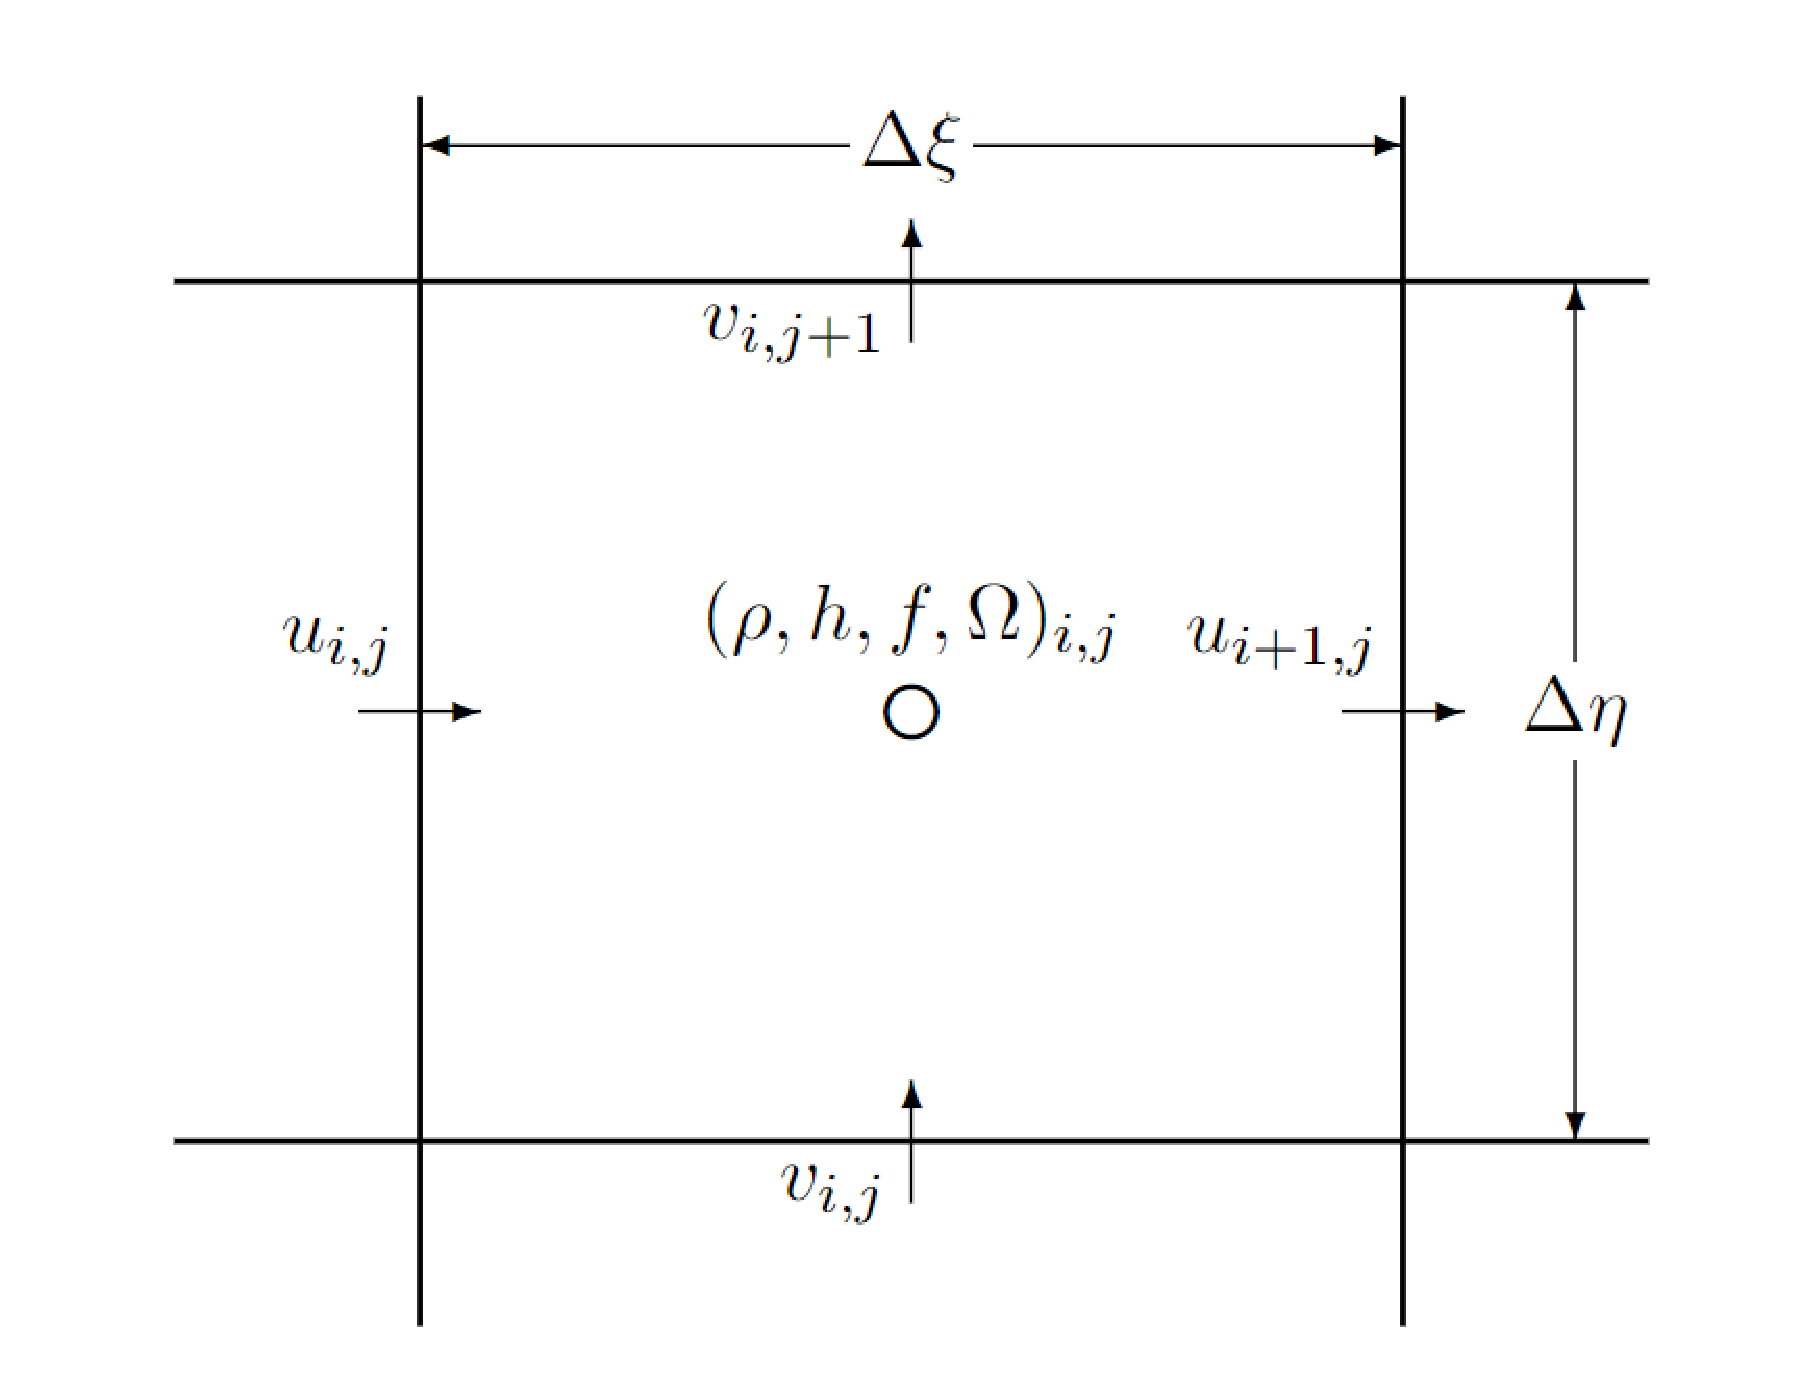
\includegraphics[width=12cm]{cgrid.eps}
        \caption{ Placement of variables on an Arakawa C grid}
    \end{figure}
    注意与流速点对应的格点遵循西南约定而其他很多有名的模型则使用东北约定.
    \subsubsection{Vertical grid}
    垂向离散采用二阶有限差分近似,与交错的水平网格相似,垂向网格也采用交错排列:
    \begin{figure}[H]
        \centering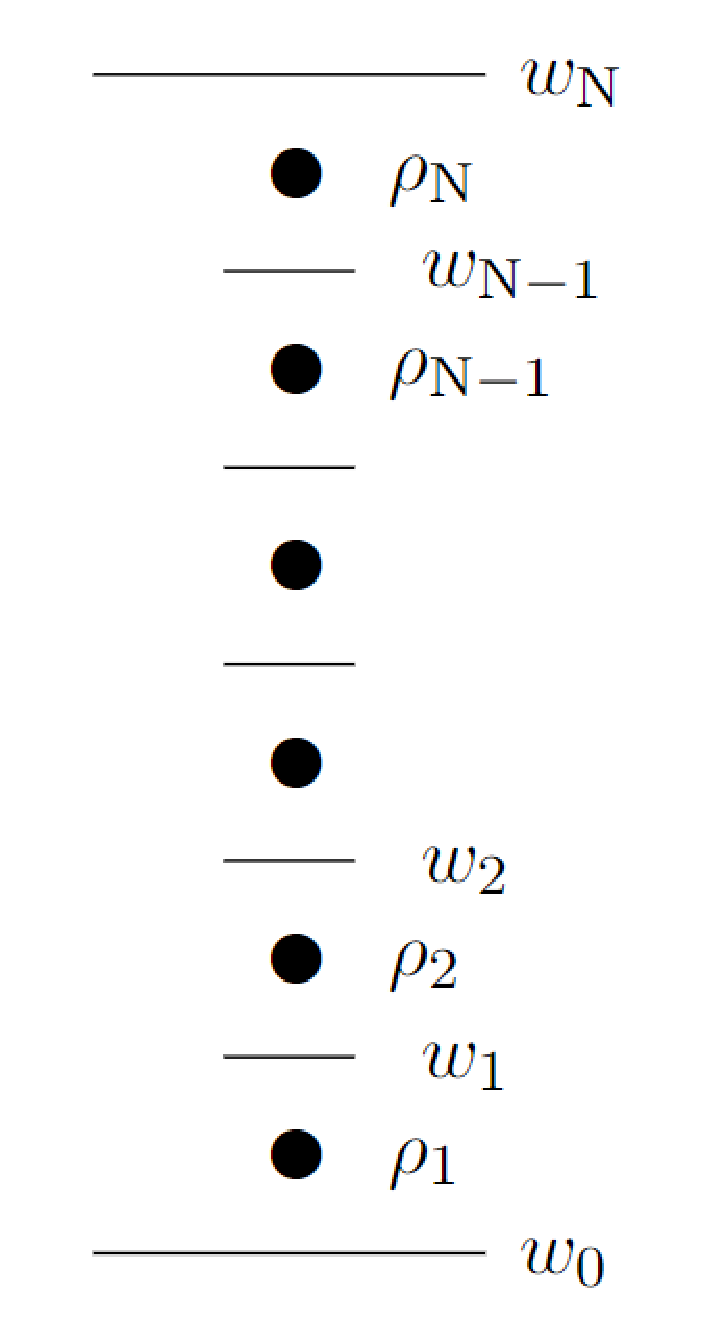
\includegraphics[width=4cm]{vertical.eps}
        \caption{Placement of variables on staggered vertical grid}
    \end{figure}
    \subsection{Masking of land areas}
    ROMS支持内部的陆地区域,本节将说明mask如何影响不同项的计算.
    \subsubsection{Velocity}

\end{document}